% =====================================================================
% Dissertation (single-column, report class) --- main file.
% Self-contained: compiles on Overleaf or any TeX Live that has the packages
% below (no CVPR style involved). This wrapper makes Method appear as
% "Chapter 4" and pulls in sec/method.tex.
% =====================================================================

\documentclass[12pt,a4paper,oneside]{report}

\usepackage[T1]{fontenc}
\usepackage[utf8]{inputenc}
\usepackage{lmodern}
\usepackage[margin=1in]{geometry}

\usepackage{amsmath,amssymb}
\usepackage{booktabs}
\usepackage{algorithm}
\usepackage{algpseudocode}
\usepackage{svg}               % \includesvg — Overleaf runs Inkscape automatically
\usepackage{graphicx}
\usepackage{microtype}
% Safety valve: lets TeX stretch a line rather than overflow the margin
% when an unbreakable token (e.g. \texttt{qwen-plus-latest}) lands badly.
\setlength{\emergencystretch}{3em}

\usepackage[hidelinks]{hyperref}
\usepackage[capitalize]{cleveref}   % load AFTER hyperref
\crefname{algorithm}{Algorithm}{Algorithms}
\Crefname{algorithm}{Algorithm}{Algorithms}

\title{Scene Graphs as Evidence Indexes:\\
       Lazy Memory and Confidence-Driven LLM Agents\\
       for Long-Video Question Answering}
\author{Your Name}
\date{}

\begin{document}
\maketitle
\tableofcontents

% --- Earlier chapters are stubs. The source outline puts Method as Chapter 4,
% --- so we advance the chapter counter to 3; the next \chapter becomes "4".
% --- Replace this with your real Chapters 1--3. The Method section
% --- cross-references two labels defined in OTHER chapters:
% ---   \label{ch:diagnosis} -> Ch.3 (baseline & diagnosis)
% ---   \label{ch:eval}      -> Ch.5 (evaluation)
% --- Until those chapters exist, \cref to them renders as "??" (normal placeholder).
\setcounter{chapter}{3}

% !TEX root = ../main.tex
% =====================================================================
% Chapter 4 (Method) --- DISSERTATION version (single-column report class).
% Converted from docs/thesis/ch4_method.md. Body text kept VERBATIM;
% only markdown->LaTeX formatting and chapter/section commands changed.
% This version preserves the "Chapter 4 / 4.1 / 4.2" numbering of the source.
%
% Placeholder cross-reference labels (live in OTHER chapters, not yet written):
%   ch:diagnosis -> Ch.3 baseline & empirical diagnosis
%   ch:eval      -> Ch.5 evaluation
% \cref to an undefined label renders as "??" until that chapter exists --- expected.
%
% Honesty red-lines preserved from source (do NOT "strengthen" these):
%   - exploration budget (<=2/round, <=3 rounds) is an INSTRUCTED budget; the
%     only enforced hard cap is recursion_limit = 40 (Lambda = 5K+10).
%   - cross-batch entity alignment threshold is difflib 0.85 (not the
%     reserved-but-unused 0.9).
%   - L0 summary uses 8 frames (hard-coded); the VLM is qwen-vl-plus.
% =====================================================================

\chapter{Method: Lazy Three-Layer Memory and Confidence-Driven Orchestration}
\label{ch:method}

\section{Overview}
\label{sec:overview}

\subsection{Problem setup and notation}
\label{subsec:setup}

We address long-video question answering: given a video $V$ of duration $T$ (roughly 20 s to
6 min in our evaluation setting; \cref{ch:eval}) and a natural-language question $q$, produce an answer $a$
that is \emph{grounded in evidence extracted from $V$}. The system operates under a perception budget:
every look at the video --- whether a set of sampled frames or a single frame --- costs one call to a
vision--language model (VLM), and the central design question of this thesis is \emph{where} those calls
should be spent. We accordingly measure the per-question perception cost as
%
\begin{equation}
\label{eq:cost}
C(q) \;=\; \#\textsc{Explore}(q) \;+\; \#\textsc{Inspect}(q)
\end{equation}
%
VLM calls (equivalently, the frames those calls consume), on top of a once-per-video $L_0$
initialisation of a single VLM call; \cref{ch:eval} reports both calls and frames per question under this
definition.

Throughout this chapter we use the following notation. The system maintains an external memory
%
\begin{equation}
\label{eq:mem}
\mathcal{M} \;=\; \langle L_0,\; L_1,\; L_2 \rangle,
\end{equation}
%
whose three layers are defined in \cref{sec:memory}: a global layer $L_0$ (one-off, cheap), an evidence layer
$L_1$ of densely captioned segments $s_i$ (built on demand), and an index layer $L_2$ of
timestamped triplets $\tau$ with provenance links back to $L_1$. A segment is a tuple
$s_i = (\mathrm{id}_i,\, t_i^{s},\, t_i^{e},\, c_i,\, F_i)$ with time window $[t_i^s, t_i^e]$,
dense caption $c_i$, and sampled frames $F_i$; a triplet is a five-tuple
$\tau = \langle \mathit{subj},\, \mathit{rel},\, \mathit{obj},\, t^{s},\, t^{e} \rangle$ with a
provenance tag $\sigma(\tau)$ identifying the segment it was extracted from. The agent interacts
with $\mathcal{M}$ exclusively through three tools --- $\textsc{Search}$ (free), $\textsc{Explore}$
(one VLM call over at most 6 frames), and $\textsc{Inspect}$ (one VLM call over a single frame) ---
under a bounded interaction budget (\cref{sec:orchestration}). While answering one question the agent accumulates an
evidence set $E$ --- the union of tool results returned so far --- and maintains a self-assessed
confidence $\gamma \in \{1, 2, 3\}$ that $E$, together with the $L_0$ context, suffices to answer
$q$; both are given operational meaning in \cref{sec:orchestration}.

\subsection{Design requirements}
\label{subsec:requirements}

\Cref{ch:diagnosis} diagnosed two failure modes of the scene-graph-centric baseline (v1): triplets used as
the \emph{answer source} form a lossy bottleneck (on-screen text, attribute detail and causal narration
are discarded at the ``emit JSON triplets'' step), and a \emph{full upfront} graph build never amortises
at the observed load of roughly one question per video. Inverting these failures yields three
requirements that the present design satisfies by construction:

\begin{itemize}
  \item \textbf{R1 --- Memory must be multi-granular and built on demand.} Cheap global context is acquired
  once; expensive dense perception is a per-question decision, spent only where a question demands
  it (\cref{sec:memory,sec:orchestration}).
  \item \textbf{R2 --- Evidence must be preserved verbatim.} Structured representations may \emph{locate} evidence
  but must never \emph{replace} it: retrieval returns the original captions and narration text, not
  their compressed surrogates (\cref{subsec:provenance}).
  \item \textbf{R3 --- Orchestration must be confidence-driven.} Whether to spend another perception call is
  decided at run time from the agent's own assessment of evidence sufficiency, under an explicit
  budget, rather than by a fixed pipeline (\cref{sec:orchestration}).
\end{itemize}

\subsection{Architecture and question lifecycle}
\label{subsec:lifecycle}

\Cref{fig:arch} shows the architecture. A \texttt{VideoSession} object owns the memory $\mathcal{M}$ for one
video; the agent --- a tool-calling LLM loop in the ReAct tradition \cite{yao2023react} --- holds no
state of its own, and every tool reads and writes the session (\cref{sec:impl}).

\begin{figure}[t]
  \centering
  % Figure is a PDF pre-converted from fig/ch4_architecture.svg (rsvg-convert -f pdf).
  % Using the PDF avoids invoking Inkscape on every compile: much faster on
  % Overleaf, and it works in any TeX install without shell-escape.
  % SVG fallback: keep \usepackage{svg} and swap this line back to
  %   \includesvg[inkscapelatex=false,width=0.85\linewidth]{fig/ch4_architecture}
  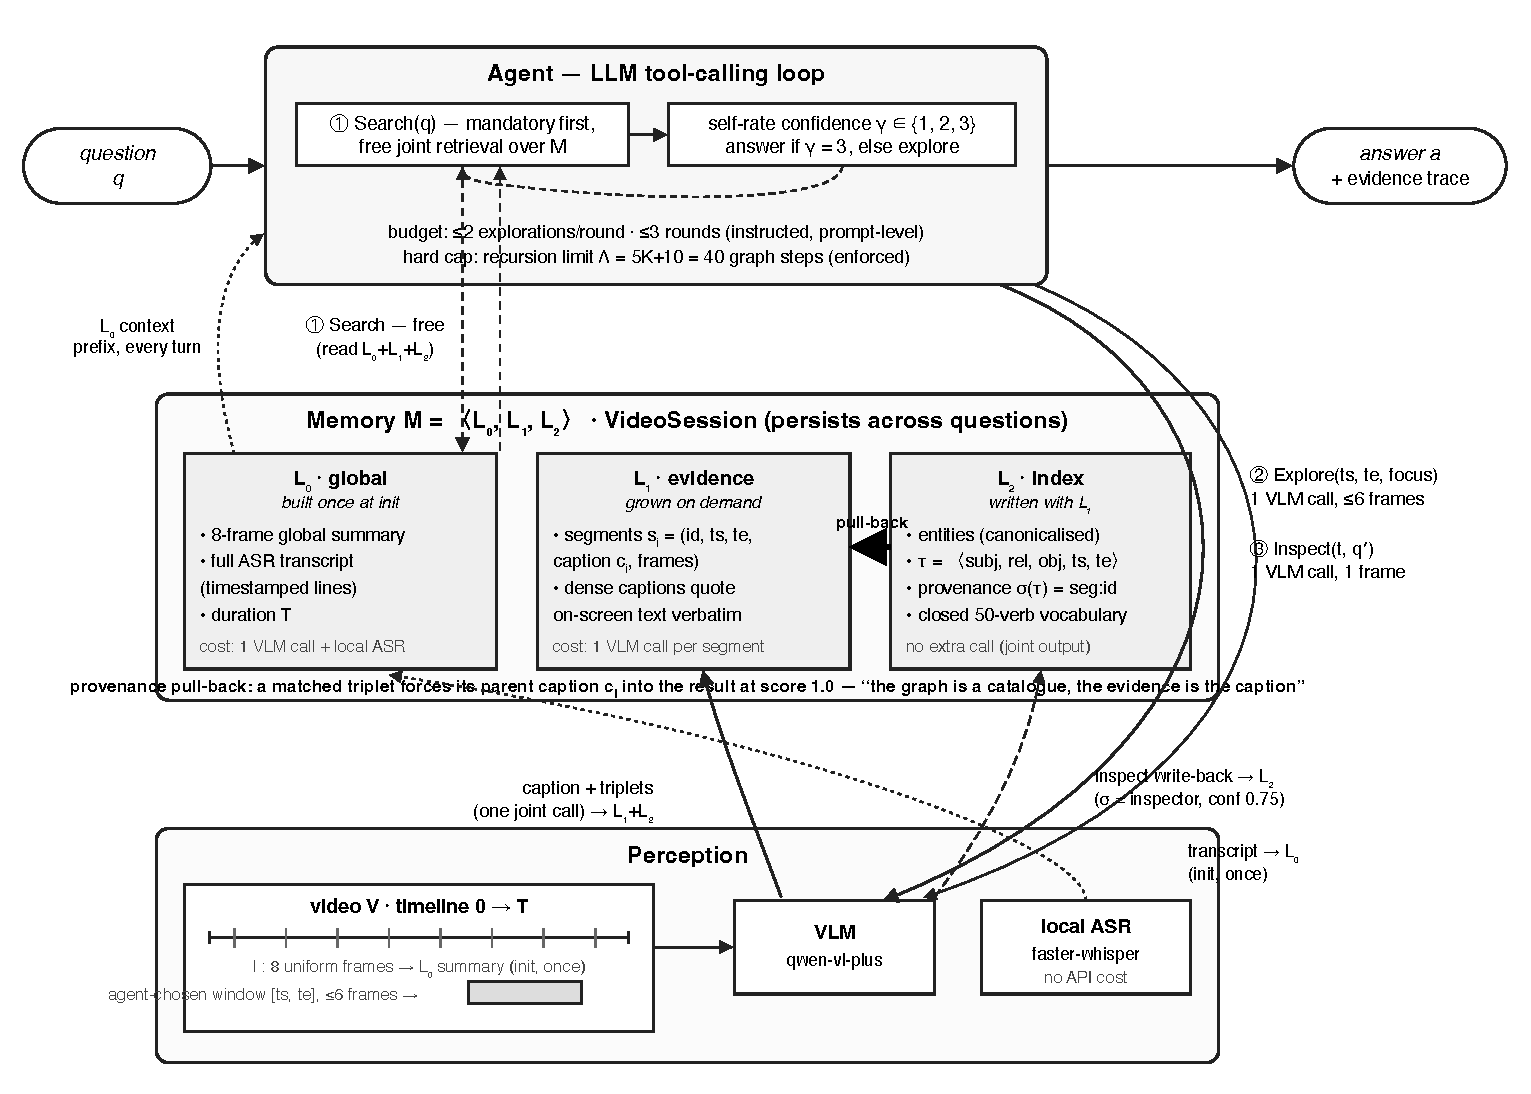
\includegraphics[width=0.85\linewidth]{fig/ch4_architecture}
  \caption{System architecture.}
  \label{fig:arch}
\end{figure}

The lifecycle of one question proceeds as follows. (1) At session creation, $L_0$ is initialised
once: a global summary from 8 uniformly sampled frames and a full narration transcript from local
ASR (\cref{subsec:l0}). (2) When $q$ arrives, an $L_0$-derived context prefix is prepended to the prompt and
the agent must first call $\textsc{Search}$, a zero-cost joint lookup over all three layers
(\cref{subsec:search}). (3) The agent privately rates the sufficiency of the returned evidence on a 1--3 scale;
if insufficient, it selects a time window and calls $\textsc{Explore}$, which performs one VLM
call over at most 6 frames and \emph{writes} a new dense caption into $L_1$ together with its indexed
triplets into $L_2$ (\cref{subsec:explore}). (4) Questions demanding pixel-level detail (on-screen text, exact
counts) may use $\textsc{Inspect}$ on a single frame, whose findings are written back into $L_2$
(\cref{subsec:inspect}). (5) The loop terminates when confidence reaches 3 or the budget is spent, and the agent
answers strictly from accumulated evidence (\cref{sec:orchestration}). Because $\mathcal{M}$ persists across
questions, later questions on the same video frequently succeed at step (2) with no further
perception cost.

\section{Lazy Three-Layer Memory}
\label{sec:memory}

\begin{table}[t]
  \centering
  \small
  \caption{The three memory layers.}
  \label{tab:layers}
  \begin{tabular}{@{}p{0.10\linewidth}p{0.32\linewidth}p{0.26\linewidth}p{0.22\linewidth}@{}}
    \toprule
    Layer & Contents & Built when & Cost \\
    \midrule
    $L_0$ global & 8-frame global summary; full timestamped ASR transcript; duration $T$ & once at session init (idempotent) & 1 VLM call + local ASR (no API cost) \\
    $L_1$ evidence & segments $s_i$ with dense captions $c_i$ (3--5 sentences, on-screen text quoted) & on demand, per $\textsc{Explore}$ call & 1 VLM call per segment ($\leq 6$ frames) \\
    $L_2$ index & entities; triplets $\tau$ with provenance $\sigma(\tau)$; closed 50-relation vocabulary & written together with $L_1$ (and by $\textsc{Inspect}$) & no extra call (joint output of the $L_1$ call) \\
    \bottomrule
  \end{tabular}
\end{table}

\subsection{$L_0$: the global layer}
\label{subsec:l0}

$L_0$ answers the question ``what is this video about, and what is said in it'' at the lowest
possible cost, so that many questions never need dense perception at all.

\textbf{Global summary.} Eight frames are sampled uniformly over $[0, T]$ and passed to the VLM in a
single call with a factual-summary instruction (setting, people, main activities in rough order,
prominent on-screen text; 3--5 sentences). On VLM failure the summary degrades to the empty string
rather than to fabricated content --- a system-wide \emph{fail-loud} contract (\cref{sec:impl}).

\textbf{Narration transcript.} The full audio track is transcribed locally with faster-whisper --- a
CTranslate2 reimplementation of Whisper \cite{radford2023whisper} --- using model size \emph{small}, int8
quantisation on CPU, and voice-activity detection, yielding rows
$(t^{s}, t^{e}, \mathit{text})$. Transcription is disk-cached per video and incurs no API cost.
The transcript is rendered into the context as timestamped lines under a budget of 12,000
characters; when a long video exceeds the budget, the head and tail are kept (60\%/40\%) and the
middle elided. The head/tail policy is empirically motivated: procedural and conclusive content ---
``what happened in the end'', final steps, outcomes --- concentrates at the ends of the track, and an
earlier truncate-the-tail policy was observed to lose exactly those questions.

\textbf{Context injection.} Every question's prompt is prefixed with an $L_0$-derived context block:
duration, global summary, the (budgeted) transcript, and --- once any exploration has happened ---
the list of already-explored windows. The prefix is recomputed from the session for each incoming
question, so it reflects the memory state left by all earlier questions rather than any
conversation history (\cref{sec:impl}).

\subsection{$L_1$: the evidence layer}
\label{subsec:l1}

$L_1$ is a growing set of \emph{segments}. Each $\textsc{Explore}(t^{s}, t^{e}, \mathit{focus})$ call
samples at most 6 frames uniformly within the chosen window and issues \textbf{one} multi-image VLM
call that produces \emph{both} outputs of the perception step jointly: a dense caption $c_i$ (3--5
sentences describing actions in order, enumerating visible objects, quoting any on-screen text
exactly) and the structured entities/relations that index it (\cref{subsec:l2}). Producing caption and
triplets in one call is deliberate: relative to issuing separate captioning and extraction calls
it halves the perception cost of a segment, and it guarantees by construction that every triplet
has a caption to point back to.

The caption is the \emph{evidence payload} of the layer --- it is what retrieval ultimately returns to
the agent (R2). The segment also records its window, its focus string, and its frame identifiers,
which makes each piece of evidence auditable down to the frames it was derived from.

\subsection{$L_2$: the temporal triplet index}
\label{subsec:l2}

$L_2$ contains an entity store and a triplet list. Entities carry a name, a type
(object/person/place/other), free-form attributes, and first/last-seen timestamps. Triplets are
five-tuples $\tau = \langle \mathit{subj}, \mathit{rel}, \mathit{obj}, t^{s}, t^{e} \rangle$ with
two metadata fields: a confidence score and a provenance tag $\sigma(\tau)$ --- \texttt{seg:<id>} for
triplets extracted by $\textsc{Explore}$, \texttt{inspector} for those written back by
$\textsc{Inspect}$. Duplicate triplets are collapsed on the key
$(\mathit{subj}, \mathit{rel}, \mathit{obj}, t^{s}, t^{e})$.

\textbf{Closed relation vocabulary.} Relations are constrained to a closed set $\mathcal{R}$ of 50
verbs (e.g. \emph{holding}, \emph{walking\_toward}, \emph{talking\_to}, \emph{placed\_on}), organised in 9 semantic
groups. The VLM prompt injects $\mathcal{R}$ with a hard instruction to choose labels only from
the list. A closed vocabulary trades recall on long-tail relations for index consistency --- the
same physical relation always receives the same label, which keyword retrieval (\cref{subsec:search}) depends
on.

\textbf{Entity-name canonicalisation (three defences).} The same person or object must map to one node
across independently processed segments; naming drift would fragment the index. Three defences
apply in order of increasing cost:

\begin{enumerate}
  \item \emph{Prevention at generation time}: the extraction prompt includes a \texttt{[Known entities]} block
  listing up to 20 existing graph entities with the instruction to reuse their exact names ---
  drift that never happens costs nothing to repair.
  \item \emph{In-batch deduplication}: within one extraction batch, entities are canonicalised on the key
  (lower-cased label, type), merging attributes and widening first/last-seen spans.
  \item \emph{Cross-batch alignment}: new labels are matched against the existing graph by string
  similarity (difflib ratio $\geq 0.85$, same type) and merged into the existing node, with the
  rename propagated to all relations in the batch.
\end{enumerate}

\textbf{Temporal merging.} Relations that share $(\mathit{subj}, \mathit{rel}, \mathit{obj})$ and whose
intervals are within a 3.0 s gap are merged into one triplet (interval union, confidence maximum);
after merging, \emph{all} edges with confidence below 0.75 are discarded (a missing confidence defaults
to 0.75 and is therefore retained). This keeps the index compact under continuous
activity --- ``person holding cup'' observed on adjacent frames becomes one interval, not a triplet
per frame.

\subsection{The provenance principle: the graph is a catalogue, not the answer}
\label{subsec:provenance}

$L_2$ exists to \emph{locate} evidence, never to \emph{be} the evidence. Mechanically: when retrieval
matches a triplet $\tau$ with $\sigma(\tau) = \texttt{seg:}i$, the parent segment's full caption
$c_i$ is forced into the result set at maximum relevance (score 1.0), regardless of whether the
caption itself matched the query. The structured fact serves as a timestamped pointer; what the
agent actually reads is the original dense description (and, through $L_0$, the narration around
that window). This single mechanism is the difference between v2 and the failed v1 design: both
build scene graphs, but v1 answered \emph{from} the graph while v2 answers \emph{through} it. The
information lost by compressing perception into $\langle \mathit{subj}, \mathit{rel},
\mathit{obj}\rangle$ tuples is recovered at retrieval time by construction.

\section{The Memory Interface: Three Tools}
\label{sec:tools}

The agent never touches frames, files or the graph directly; it acts through three tools that
read or grow $\mathcal{M}$. \Cref{tab:tools} summarises their contracts.

\begin{table}[t]
  \centering
  \footnotesize
  \caption{Tool contracts.}
  \label{tab:tools}
  \setlength{\tabcolsep}{4pt}
  \begin{tabular}{@{}llp{0.30\linewidth}p{0.17\linewidth}l@{}}
    \toprule
    Tool & Input & Returns & Cost & Writes \\
    \midrule
    $\textsc{Search}$ & question text & matched triplets, segment captions, transcript lines, entity summary, explored windows & \textbf{free} (no API call) & --- \\
    $\textsc{Explore}$ & window $[t^{s}, t^{e}]$, focus & new segment id, caption, graph deltas, updated explored windows & 1 VLM call ($\leq 6$ frames) & $L_1$ + $L_2$ \\
    $\textsc{Inspect}$ & timestamp, sub-question & pixel-level answer, entities/relations found & 1 VLM call (1 frame) & $L_2$ \\
    \bottomrule
  \end{tabular}
\end{table}

\subsection{$\textsc{Search}$: free joint retrieval}
\label{subsec:search}

$\textsc{Search}(q)$ performs keyword retrieval jointly over all three layers. Query and memory
text are tokenised identically: lower-cased, split on alphanumerics, stop-words removed, and each
token lemmatised against WordNet \cite{miller1995wordnet} (via NLTK \cite{bird2009nltk}) --- verb reading
first, then noun --- so that surface variants match (``cooking'' $\approx$ ``cooks'' $\approx$ ``cook''). When the
WordNet data is unavailable (fully offline deployments), lemmatisation degrades to a lightweight
suffix-stripping stemmer; all reported experiments used the WordNet path.

\begin{itemize}
  \item \textbf{Over $L_2$} (top 5, minimum score 0.3): a triplet is scored by summed keyword weights
  %
  \begin{equation}
  \label{eq:score}
  \begin{aligned}
  \mathrm{score}(\tau, q) &\;=\; \sum_{t \,\in\, \mathrm{tok}(q)} w(t, \tau), \\[2pt]
  w(t, \tau) &\;=\; \begin{cases}
  2.0 & t = \mathit{subj} \ \text{or}\ t = \mathit{obj} \\
  1.5 & t = \mathit{rel} \\
  0.5 & t \sqsubset \mathit{subj} \ \text{or}\ t \sqsubset \mathit{obj} \\
  0.3 & t \sqsubset \mathit{rel} \\
  0 & \text{otherwise,}
  \end{cases}
  \end{aligned}
  \end{equation}
  %
  where $\sqsubset$ denotes proper substring containment and the first matching case applies.
  Temporal phrases in the question additionally filter by time: ``at the beginning/first''
  restricts to the first 20\% of $[0,T]$, ``at the end/last'' to the final 20\%, and an explicit
  second/minute reference to a $\pm 3$ s ($\pm 5$ s) neighbourhood.
  \item \textbf{Over $L_1$} (top 3): captions score by query-token coverage
  $\mathrm{cov}(c_i, q) = |\mathrm{tok}(q) \cap \mathrm{tok}(c_i)| \,/\, |\mathrm{tok}(q)|$,
  plus the provenance pull-back of \cref{subsec:provenance}.
  \item \textbf{Over $L_0$} (top 4): each transcript line scores by the same coverage measure
  $\mathrm{cov}(\cdot, q)$.
\end{itemize}

A minimum score of 0.15 filters segment and transcript hits. The result also reports the current
explored windows, so the agent can reason about \emph{where memory has not looked yet} --- the basis of
the grounding rule in \cref{subsec:grounding}. Because $\textsc{Search}$ is free, the orchestration policy can
mandate it unconditionally as the first action of every question.

\subsection{$\textsc{Explore}$: on-demand dense perception}
\label{subsec:explore}

$\textsc{Explore}$ is the only operation that grows the evidence base, implementing R1's ``build
on demand''. The agent chooses the window itself --- guided by the transcript timestamps, the
question's temporal cues, and the gaps in explored windows --- which is precisely what
distinguishes \emph{guided} sampling from the uniform sampling of direct-VLM baselines (\cref{ch:eval} quantifies
this difference). The tool contract advises windows of 10--30 s; a degenerate window below 0.5 s
falls back to a single frame.

\subsection{$\textsc{Inspect}$: single-frame pixel reading}
\label{subsec:inspect}

$\textsc{Inspect}(t, q')$ answers a focused sub-question on the single frame nearest to $t$.
Frame selection degrades in three stages: a cached frame within a 2 s tolerance is preferred;
failing that, the frame is extracted from the video on demand; and if extraction itself fails
(e.g. the source file is no longer accessible), the tool falls back to the temporally nearest
cached frame regardless of tolerance, disclosing the timestamp actually used in its result.
It exists because
some evidence --- exact on-screen wording, small object counts --- survives neither summarisation nor
6-frame segment captioning. Entities and relations discovered during inspection are written back
into $L_2$ (provenance \texttt{inspector}, confidence 0.75), so pixel-level findings become retrievable
by later questions. If the frame cannot be read or the backend is unavailable, the tool returns
an explicit error rather than a guess (\cref{sec:impl}).

\section{Confidence-Driven Orchestration}
\label{sec:orchestration}

\subsection{The loop}
\label{subsec:loop}

The orchestration policy is stated to the agent as a procedure and realised as a tool-calling LLM
loop (\cref{alg:loop}). The agent must open with $\textsc{Search}$; it then privately rates the
sufficiency of available evidence on a three-point scale --- 1 (insufficient), 2 (partial), 3
(sufficient) --- and, while below 3, gathers evidence with $\textsc{Explore}$ under an instructed
budget of at most 2 explorations per round and 3 rounds in total. The loop stops as soon as
confidence reaches 3 or the budget is spent, and the agent must then give its best \emph{supported}
answer --- or state what evidence is missing, rather than guess.

\begin{algorithm}[t]
\caption{Confidence-driven answering (one question).}
\label{alg:loop}
\begin{algorithmic}[1]
\Require question $q$, session memory $\mathcal{M} = \langle L_0, L_1, L_2 \rangle$
\Ensure answer $a$ grounded in $\mathcal{M}$
\State $E \gets \textsc{Search}(q)$ \Comment{[system] mandatory first action; free}
\For{round $r = 1..3$} \Comment{instructed budget (see \cref{subsec:budget})}
    \State $\gamma \gets$ self-rate confidence of $(E,\, L_0\text{-context}) \in \{1, 2, 3\}$ \Comment{[LLM]}
    \If{$\gamma = 3$} \State \textbf{break} \EndIf
    \State $j \gets 0$
    \While{$\gamma < 3$ \textbf{and} $j < 2$} \Comment{up to 2 explorations per round}
        \State $[t_s, t_e] \gets$ choose window \Comment{[LLM] transcript cues, temporal phrases, gaps in explored windows}
        \State $E \gets E \cup \textsc{Explore}(t_s, t_e, \mathit{focus})$ \Comment{[system] writes $L_1 + L_2$}
        \State $\gamma \gets$ re-rate confidence on the new evidence \Comment{[LLM]}
        \State $j \gets j + 1$
    \EndWhile
    \State (optional) $E \gets E \cup \textsc{Inspect}(t, q')$ \Comment{[LLM] pixel-level detail}
\EndFor
\State $a \gets$ answer from $E$ and $L_0$-context only \Comment{grounding rules, \cref{subsec:grounding}}
\end{algorithmic}
\vspace{3pt}
{\footnotesize
$\triangleright$~[system] the whole loop runs under an enforced recursion cap $\Lambda = 5K+10 = 40$.\par
$\triangleright$~lines tagged [LLM] are model decisions instructed by the system prompt;
lines tagged [system] are enforced by the orchestration code.\par}
\end{algorithm}

\subsection{Instructed budget versus enforced cap}
\label{subsec:budget}

The budget in \cref{alg:loop} (lines 2 and 6) is \emph{instructed}: it is part of the system prompt, and
the model is trusted to follow it. It is not enforced by a counter in code. The \emph{enforced}
bound is the orchestration framework's recursion limit $\Lambda = 5K + 10 = 40$ graph steps,
where $K = 6$ is the framework-level iteration allowance carried in the configuration --- a
quantity distinct from, and deliberately looser than, the three instructed rounds. The factor
five is a heuristic per-round upper bound (one model call, up to two tool invocations and their
returns) and the constant term adds headroom for the initial and final exchanges; $\Lambda$ is
intentionally generous, because the tight constraint is meant to be the instructed budget, not
the cap. In the runs=3 benchmark campaign (\cref{ch:eval}), no question exhausted
$\Lambda$, and observed behaviour stayed within the instructed budget (mean 1.7 tool calls and
3.6 frames per question); we nevertheless report the budget as instructed rather than enforced,
because that is what the implementation guarantees.

\subsection{Grounding rules}
\label{subsec:grounding}

Three rules connect confidence to \emph{evidence} rather than to the model's parametric knowledge:

\begin{enumerate}
  \item \textbf{Absence is not ``no''.} Memory covers only explored windows; failing to find a fact in
  $\mathcal{M}$ is not evidence of its absence in $V$. Before answering ``no'', the agent must
  explore the relevant window. This rule is the mechanism behind the hallucination-resistance
  results of \cref{ch:eval}: fabricating an answer about unexplored content is procedurally disallowed.
  \item \textbf{The transcript is authoritative for narration.} Questions about reasons, methods, spoken
  content or step order are answered from ASR text with visual confirmation, not from visual
  inference alone.
  \item \textbf{No parametric answers.} The final answer must derive from retrieved or newly gathered
  evidence and the $L_0$ context; if the budget expires with insufficient evidence, the agent
  states what is missing.
\end{enumerate}

Two auxiliary window-selection heuristics are instructed alongside: a short video ($\lesssim$60 s)
with nothing explored should be explored in full first; and duration or order comparisons require
the complete extent of the events involved --- if a fact's interval touches the edge of an explored
window, the window is widened before concluding.

\subsection{Answer modes and robustness}
\label{subsec:modes}

The same agent runs in two answer modes: a benchmark mode constrained to short answers (single
word or phrase; exact ``yes''/``no'') and a product mode producing 1--3 sentences with timestamps.
Two robustness mechanisms wrap the loop. First, small open-weight models occasionally emit a
tool call as plain text instead of a structured call; a pattern detector catches such
``pseudo-calls'' on the final message and re-asks once with a corrective instruction. Second, VLM
JSON output is parsed with three-level tolerance (direct parse; outermost-braces extraction;
bracket-depth array salvage for the entity/relation lists), recovering the caption from free text
when structure is mangled. Failures that survive all defences degrade loudly --- empty results and
explicit error payloads --- never silently into fabricated content.

\section{Implementation Notes}
\label{sec:impl}

The agent is built on LangChain's \texttt{create\_agent} (LangGraph runtime; \cite{langchain2022}) with the tool
set of \cref{tab:tools}; the backbone LLM is Qwen (the DashScope \texttt{qwen-plus-latest} alias in all
reported experiments; a local vLLM backend is interface-compatible), and the VLM is
\texttt{qwen-vl-plus}, with images resized to a 1280 px longest edge. Both are hosted models behind
rolling aliases that cannot be pinned to a fixed snapshot; all experiments were run within a
single access window (June--July 2026), and this limitation is revisited among the threats to
validity in \cref{ch:eval}. All durable state lives in the \texttt{VideoSession} --- the LangGraph message list
is not reused across questions; each question starts a fresh conversation whose only continuity
is the session memory itself. This externalisation keeps prompt length constant in the number of
questions, makes memory growth explicit (only $\textsc{Explore}$/$\textsc{Inspect}$ write), and
gives multi-turn reuse for free: consecutive questions about neighbouring content typically
resolve at $\textsc{Search}$ time with zero perception cost.

Reliability follows a \emph{fail-loud} contract used throughout: mock/offline paths are visually
labelled and never fabricate domain data; real-path failures return explicit error markers
(degrading, e.g., to a missing summary or an empty transcript) instead of synthetic evidence that
could contaminate answers or evaluation. All token and call counts reported in \cref{ch:eval} come from a
thread-safe usage ledger recording the API-reported usage of every call --- no estimates. VLM calls
carry six retries with a 90 s timeout; the ASR transcript is disk-cached per video and reused
across runs and sessions.

\Cref{tab:constants} consolidates every constant used in this chapter, with its provenance: \emph{hard-coded}
(fixed in source), \emph{config default} (exposed in the layered configuration but left at its
default), or \emph{prompt-instructed} (stated to the model, not enforced in code). All values were
frozen before the evaluation campaign reported in \cref{ch:eval}; none were tuned against the benchmark
after that point.

\begin{table}[t]
  \centering
  \small
  \caption{Constants and hyperparameters (verified against the implementation).}
  \label{tab:constants}
  \begin{tabular}{@{}p{0.42\linewidth}p{0.34\linewidth}p{0.18\linewidth}@{}}
    \toprule
    Constant & Value & Provenance \\
    \midrule
    $L_0$ summary frames & 8, uniform & hard-coded \\
    ASR model & faster-whisper \emph{small}, int8, VAD & hard-coded \\
    Transcript context budget & 12,000 chars (60\% head / 40\% tail) & hard-coded \\
    $\textsc{Explore}$ frames per window & $\leq 6$, uniform & hard-coded \\
    Exploration budget & $\leq 2$ per round, $\leq 3$ rounds & prompt-instructed \\
    $\textsc{Inspect}$ frame tolerance & 2.0 s & config default \\
    $\textsc{Inspect}$ write-back confidence & 0.75 & config default \\
    Relation vocabulary & 50 verbs / 9 groups & hard-coded \\
    \texttt{[Known entities]} prompt block & $\leq 20$ entities & hard-coded \\
    Cross-batch name alignment & difflib ratio $\geq 0.85$, same type & hard-coded\textsuperscript{1} \\
    Temporal merge gap & $\leq 3.0$ s & config default \\
    Edge confidence filter & $\geq 0.75$ & config default \\
    $\textsc{Search}$ weights $w$ & 2.0 / 1.5 / 0.5 / 0.3 & hard-coded \\
    $\textsc{Search}$ top-$k$ ($L_2$/$L_1$/$L_0$) & 5 / 3 / 4 & hard-coded \\
    $\textsc{Search}$ minimum scores & 0.3 (triplets); 0.15 (captions, transcript) & hard-coded \\
    Provenance pull-back score & 1.0 & hard-coded \\
    Time-phrase filters & first/last 20\%; $\pm 3$ s ($\pm 5$ s for minutes) & hard-coded \\
    Iteration allowance $K$ / cap $\Lambda$ & 6 / 40 (= 5K+10) & config default / derived \\
    VLM retries / timeout & 6 / 90 s & hard-coded \\
    Image longest edge & 1280 px & config default \\
    \bottomrule
  \end{tabular}

  \vspace{2pt}
  {\footnotesize \textsuperscript{1} A \texttt{dedup\_threshold: 0.9} field exists in the configuration but is reserved for a future
  embedding-based deduplication and is not wired to this path; the operative value is 0.85.}
\end{table}


% !TEX root = ../main.tex
% =====================================================================
% Chapter 5 (Evaluation) --- DISSERTATION version (single-column report class).
% Written from the repository's canonical result documents; every number is
% sourced (no numbers from memory):
%   - docs/reviews/project_review_202607.md  §1.4  (canonical number memo)
%   - docs/analysis/benchmark_mmbv_final_analysis.md  (closing analysis)
%   - docs/results/benchmark_mmbv_final_gpt4judge.md  (paper-setting dimension tables)
%   - docs/results/benchmark_mmbv_final_official_agg.md  (qwen-max robustness control)
%   - docs/results/benchmark_mmbv_dense_{16f,32f}*.md  (frame-scaling)
%   - docs/results/benchmark_v2_agqa.md, annotation_audit.json
%   - docs/progress.md  §14.1 / §14.2 / §14.3 / §16.1 / §16.2
%
% Judge-setting discipline (from thesis_outline.md §4):
%   * paper-level and dimension-level citations = gpt-4-turbo re-judge
%     (1.978 / 1.713 / 1.491, gap 0.265; HL 2.29 vs 0.78);
%   * the runs=3 noise-robustness argument = qwen-max as-run scores with ±std
%     (1.984±0.101 / 1.727±0.020 / 1.478±0.025, gap 0.257 > std-sum 0.121);
%   * duration buckets and the attribution ladder are derived from qwen-max
%     raw scores (stated in the text).
% Honesty red-lines: frames/question is 3.6 (runs=3 authority; 3.1 was runs=1);
% the 81/69 zero-explore split is a runs=1 diagnostic figure; TR is a LOSING
% dimension and is disclosed as such; total tokens are ~2.1x the baseline (no
% cost-saving claims); the 150-question subset is NOT comparable to the public
% leaderboard; frame-scaling main protocol is common-147 (moderation-blocked
% items removed from every condition), full-150 in the appendix.
%
% Cross-references into other chapters: ch:method (exists), ch:diagnosis
% (Ch.3, not yet written -> renders "??" until then).
% =====================================================================

\chapter{Evaluation}
\label{ch:eval}

This chapter evaluates the system of \cref{ch:method} on MMBench-Video with a
protocol designed to answer three questions: whether the agent outperforms
direct-VLM baselines under honest accounting (\cref{sec:main-results}), where the
gain comes from (\cref{sec:attribution}), and what the perception budget buys
(\cref{sec:budget}). Analyses by duration and capability dimension
(\cref{sec:analysis}), falsified alternatives (\cref{sec:negative}), a transfer
check (\cref{sec:agqa}), an annotation audit with threats to validity
(\cref{sec:threats}), and two worked traces (\cref{sec:case}) complete the picture.

\section{Experimental Setup}
\label{sec:setup}

\textbf{Benchmark.} We evaluate on a 150-question subset of
MMBench-Video~\cite{fang2024mmbenchvideo} spanning 136 videos, drawn by stratified
sampling (seed 42) with deliberate oversampling of the Temporal Reasoning (TR) and
Hallucination (HL) dimensions. Because the subset re-balances the official
distribution, \emph{our scores are not directly comparable to the public
leaderboard}, which is computed on the full 1{,}998 questions; re-weighting our
per-dimension scores by the official distribution moves every method's total by at
most $0.04$ (agent $+0.017$), so the subset composition does not drive any
conclusion below.

\textbf{Scoring protocol.} We replicate the official
VLMEvalKit~\cite{duan2024vlmevalkit} protocol: an LLM judge scores each answer on a
0--3 scale (judge prompt, scale, temperature $0$, and failure handling replicated
verbatim), and dimension aggregation follows the official multi-label
\texttt{get\_dimension\_rating} (each question counts toward every capability it is
tagged with: 26 leaf capabilities, 9 L2 dimensions, and Perception/Reasoning/Overall
roll-ups). Two judges are used throughout. The as-run judge is
\texttt{qwen-max}; after the campaign, every cached answer was re-judged by
\texttt{gpt-4-turbo}~\cite{openai2023gpt4} --- the judge family used by the official
benchmark --- totalling 1{,}350 judgements. Unless stated otherwise,
\emph{paper-level and dimension-level numbers below use the gpt-4-turbo setting},
with qwen-max retained as a robustness control; the two settings agree to within
$0.015$ on every method's total, with per-question agreement 0.76--0.81. Derived
analyses (duration buckets, the attribution ladder) are computed from the qwen-max
raw scores and labelled as such.

\textbf{Systems.} Four systems are compared, all sharing the same backbone LLM
(\texttt{qwen-plus-latest}~\cite{bai2023qwen}) and VLM
(\texttt{qwen-vl-plus}~\cite{bai2023qwenvl}; cf.\ \cref{sec:impl}):
\begin{itemize}
  \item \textbf{agent\_v2} (ours): the lazy-memory, confidence-driven agent of
  \cref{ch:method}.
  \item \textbf{vlm\_direct@8}: the VLM answers directly from 8 uniformly sampled
  frames.
  \item \textbf{vlm\_transcript@8} (\emph{fair baseline}): identical to
  vlm\_direct@8 \emph{plus} the full ASR transcript in the prompt. Since the agent
  also consumes ASR, this baseline holds the input modalities fixed and isolates
  the contribution of the architecture (\cref{sec:attribution}).
  \item \textbf{v1}: the scene-graph-centric baseline diagnosed in
  \cref{ch:diagnosis} (legacy, single run).
\end{itemize}

\textbf{Runs and accounting.} The three main systems are run three times
independently (runs=3); we report mean $\pm$ standard deviation. All token, call,
and frame counts come from a thread-safe ledger recording the API-reported usage of
every call --- no estimates (\cref{sec:impl}). Beyond accuracy we report
\emph{frames-touched per question}: the number of frames the system actually sent
to the VLM for that question.

\section{Main Results}
\label{sec:main-results}

\Cref{tab:main} shows the headline result: the agent outperforms both baselines
under both judge settings.

\begin{table}[t]
  \centering
  \small
  \caption{Overall results on the MMBench-Video subset (0--3 scale, mean $\pm$ std
  over 3 runs). The gpt-4-turbo column is the paper-level setting; qwen-max is the
  as-run robustness control. v1 is the legacy baseline of \cref{ch:diagnosis}
  (single run, qwen-max).}
  \label{tab:main}
  \begin{tabular}{@{}lccc@{}}
    \toprule
    Method & Overall (gpt-4-turbo) & Overall (qwen-max) & Frames/Q \\
    \midrule
    \textbf{agent\_v2 (ours)} & $\mathbf{1.978 \pm 0.097}$ & $\mathbf{1.984 \pm 0.101}$ & \textbf{3.6} \\
    vlm\_transcript@8 & $1.713 \pm 0.019$ & $1.727 \pm 0.020$ & 8.0 \\
    vlm\_direct@8 & $1.491 \pm 0.019$ & $1.478 \pm 0.025$ & 8.0 \\
    v1 (scene-graph pipeline) & --- & 1.193 & --- \\
    \bottomrule
  \end{tabular}
\end{table}

\textbf{The reversal survives run noise.} Under the qwen-max setting the gap over
the fair baseline is $1.984 - 1.727 = 0.257$, which exceeds the \emph{sum} of the
two standard deviations ($0.101 + 0.020 = 0.121$); under gpt-4-turbo the gap widens
slightly to $0.265$. The agent's larger run-to-run variance ($\pm 0.101$ against
$\pm 0.020$ for the deterministic-sampling baselines) stems from exploration-path
randomness: at low temperature the agent may choose different windows across runs
(a concrete instance appears in \cref{sec:case}). Even so, the worst agent run
exceeds the best fair-baseline run.

\textbf{v1 confirms the diagnosis.} The scene-graph-centric v1 scores 1.193 ---
below even the 8-frame direct baseline --- reproducing the failure analysed in
\cref{ch:diagnosis}: when triplets are the \emph{answer source}, the graph is a
lossy bottleneck rather than an asset. The v2 reversal therefore cannot be
attributed to ``using a scene graph'' per se, but to using it as an index
(\cref{subsec:provenance}).

\section{Attribution: Modality versus Architecture}
\label{sec:attribution}

The fair baseline decomposes the total gain into two steps (qwen-max raw scores;
the architecture step is $0.265$ under gpt-4-turbo):

\begin{table}[h]
  \centering
  \small
  \caption{Attribution ladder (qwen-max, runs=3 means). Each step changes exactly
  one factor.}
  \label{tab:attribution}
  \begin{tabular}{@{}lccl@{}}
    \toprule
    Step & From $\to$ To & $\Delta$ & Factor isolated \\
    \midrule
    ASR modality & $1.478 \to 1.727$ & $+0.249$ & add narration text, same frames \\
    Architecture & $1.727 \to 1.984$ & $+0.257$ & same modalities, agentic memory + orchestration \\
    \bottomrule
  \end{tabular}
\end{table}

The two contributions are almost exactly equal. This rules out the deflationary
reading that the agent ``wins only because it hears the narration'': granting the
baseline the same narration still leaves a $+0.257$ gap that only the architecture
--- lazy evidence memory, provenance pull-back, and confidence-driven exploration
--- can explain. Conversely, the modality step confirms that ASR is a genuinely
load-bearing input for this benchmark, which \cref{sec:analysis} revisits when
interpreting the TR dimension.

\section{Analysis by Duration and Dimension}
\label{sec:analysis}

\subsection{Video duration: the comfort zone ends at 90 seconds}
\label{subsec:duration}

\begin{table}[t]
  \centering
  \small
  \caption{Overall score by video-duration bucket (qwen-max raw scores, runs=3
  means).}
  \label{tab:duration}
  \begin{tabular}{@{}lccc@{}}
    \toprule
    Duration bucket & agent\_v2 & vlm\_transcript@8 & vlm\_direct@8 \\
    \midrule
    $<$90\,s \hfill ($n=52$) & 1.81 & 1.76 & 1.57 \\
    90--180\,s \hfill ($n=50$) & \textbf{2.10} & 1.55 & 1.34 \\
    $>$180\,s \hfill ($n=48$) & \textbf{2.05} & 1.87 & 1.52 \\
    \bottomrule
  \end{tabular}
\end{table}

\Cref{tab:duration} locates \emph{where} the architecture pays. Below 90 seconds
the agent and the fair baseline are statistically indistinguishable (1.81 vs.\
1.76): a short video fits comfortably into 8 uniform frames plus narration, so
guided exploration has little to add. The picture inverts beyond 90 seconds ---
$2.10$ vs.\ $1.55$ at 90--180\,s and $2.05$ vs.\ $1.87$ beyond 180\,s. This is the
expected signature of the design: uniform sampling dilutes as duration grows, while
question-guided window selection does not. We accordingly describe the system's
contribution as \emph{long-video evidence localization and integration}, with
$\approx$90\,s as the boundary of the baselines' comfort zone.

\subsection{Capability dimensions}
\label{subsec:dimensions}

\begin{table}[t]
  \centering
  \small
  \caption{Per-dimension results in the MMBench-Video Table-3 layout
  (gpt-4-turbo judge, official multi-label aggregation, 0--3). \emph{P.\ Mean} /
  \emph{R.\ Mean} are the Perception / Reasoning roll-ups. Full per-dimension
  tables with standard deviations for both judge settings appear in
  \cref{app:tables}.}
  \label{tab:dimensions}
  \footnotesize
  \setlength{\tabcolsep}{3.2pt}
  \begin{tabular}{@{}lcccccccccccc@{}}
    \toprule
    Model & Overall & CP & FP-S & FP-C & HL & \emph{P. Mean} & LR & AR & RR & CSR & TR & \emph{R. Mean} \\
    \midrule
    agent\_v2 & \textbf{1.98} & \textbf{2.18} & \textbf{2.08} & \textbf{1.47} & \textbf{2.29} & \textbf{2.04} & \textbf{2.18} & 2.07 & 2.07 & 2.21 & 1.74 & 1.98 \\
    vlm\_transcript & 1.71 & 1.78 & 1.81 & 0.90 & 0.78 & 1.42 & 1.73 & \textbf{2.50} & \textbf{2.12} & \textbf{2.28} & \textbf{1.87} & \textbf{2.07} \\
    vlm\_direct & 1.49 & 1.53 & 1.64 & 0.77 & 0.64 & 1.28 & 1.39 & 2.21 & 1.81 & 2.26 & 1.52 & 1.79 \\
    \bottomrule
  \end{tabular}
\end{table}

\Cref{tab:dimensions} decomposes the gain. Three observations:

\textbf{The architectural gain is a perception gain.} The agent wins the Perception
roll-up decisively (2.04 vs.\ 1.42) while the Reasoning roll-up stays near parity
(1.98 vs.\ 2.07, a small loss): all three systems share the same backbone LLM, so
the architecture buys \emph{seeing accurately}, not thinking harder. The largest
single-dimension effects are exactly where verbatim, targeted evidence should
matter: cross-instance fine-grained perception (FP-C, 1.47 vs.\ 0.90) and
hallucination resistance below.

\textbf{Hallucination resistance is the standout mechanism.} On the HL dimension
the agent scores 2.29 against 0.78 for the fair baseline
($\approx$2.9$\times$; gpt-4-turbo setting). Under the qwen-max setting the same
comparison reads $2.42 \pm 0.19$ vs.\ $1.04$ vs.\ $0.62$
($\approx$2.3$\times$ / 3.9$\times$) --- the direction is judge-independent. We
attribute this to the grounding rules of \cref{subsec:grounding}: answering ``no''
about unexplored content is procedurally disallowed, so fabricating an answer is
replaced by either exploration or a stated lack of evidence
(\cref{sec:case} shows one such trace).

\textbf{TR is honestly lost --- and the loss is informative.} On Temporal Reasoning
the agent scores 1.74 against the fair baseline's 1.87. Note the baseline itself
jumps from 1.52 (no ASR) to 1.87 (with ASR): most of the benchmark's temporal
signal lives in the narration, i.e.\ the TR gain is \emph{modality-driven}, not
architecture-driven. This is why we frame the contribution as evidence
localization and integration rather than ``improved temporal reasoning'': on
questions whose temporal structure is already spelled out in the transcript, an
extra retrieval layer can only add noise.

\section{Perception Budget and Frame Scaling}
\label{sec:budget}

\subsection{What the agent spends}
\label{subsec:cost}

\begin{table}[t]
  \centering
  \small
  \caption{Per-question cost accounting (runs=3 means; tokens from API-reported
  usage). Prebuild = once-per-video $L_0$ initialisation amortised per question.
  Wall-clock times are from the as-run campaign.}
  \label{tab:cost}
  \footnotesize
  \setlength{\tabcolsep}{4pt}
  \begin{tabular}{@{}lcccccc@{}}
    \toprule
    Method & Tool calls & Frames/Q & Tokens/Q (answer) & + Prebuild/Q & = Total/Q & Time (s) \\
    \midrule
    agent\_v2 & 1.7 & \textbf{3.6} & 10{,}546 & 6{,}108 & 16{,}655 & 21.8 \\
    vlm\_transcript@8 & --- & 8.0 & 7{,}299 & --- & 7{,}299 & 3.4 \\
    vlm\_direct@8 & --- & 8.0 & 6{,}748 & --- & 6{,}748 & 3.7 \\
    \bottomrule
  \end{tabular}
\end{table}

\Cref{tab:cost} states the price of the reversal honestly. The agent touches
\textbf{3.6 frames per question} against the baselines' fixed 8 --- a 55\% frame
reduction --- and averages only 1.7 tool calls, evidence that the instructed budget
of \cref{subsec:budget} is respected in practice. In exchange, total token
consumption is $\approx$2.1$\times$ the fair baseline (16{,}655 vs.\ 7{,}299 per
question) and latency is $\approx$6$\times$ (21.8\,s vs.\ 3.4\,s): the agentic loop
pays in LLM tokens and wall-clock time for what it saves in perception. The value
proposition is therefore \emph{frame efficiency and long-video accuracy}, not cost
reduction.

In a single-run diagnostic breakdown, 81 of 150 questions were answered from free
retrieval alone (zero exploration) while 69 self-escalated to exploration; the
zero-exploration batch scores far higher on average (2.259 vs.\ 1.551), a gap that
\cref{sec:negative} shows to be selection bias rather than evidence that
exploration hurts.

\subsection{Frame scaling: can the baselines just look at more frames?}
\label{subsec:framescaling}

A natural objection is that the baselines are starved: give a dense sampler enough
frames and it should catch up. We test this directly by densifying both baselines
to 16 and 32 uniform frames (single run each, verbose answer mode) and judging
under both settings.

\textbf{Protocol (common-147).} Dense sampling has a hidden failure mode: three
questions (mmbv-0131, 0679, 1185) are killed by the hosting provider's content
moderation with a deterministic HTTP 400, and the error count rises monotonically
with frame count (0 errors at 8f, 1 at 16f, 3 at 32f; 100\% reproducible on
confirmatory reruns, retries ineffective --- the 8-frame baselines and the agent
score normally on all three). To avoid crediting the agent for infrastructure
failures, we remove these three questions from \emph{every} condition, including
the agent and the 8f baselines, yielding the common-147 protocol; the full-150
accounting, which scores moderation kills as 0 and therefore \emph{underestimates}
the dense baselines, is reported in \cref{app:tables}. Because the dense runs are
single-run, the curves use each system's first trial; the agent's three-run means
(qwen 1.968, gpt-4-turbo 1.957) agree with its trial-1 value in ordering.

\begin{figure}[t]
  \centering
  % Figure is a PDF pre-converted from fig/frame_scaling.svg (rsvg-convert -f pdf).
  % Using the PDF avoids invoking Inkscape on every compile: much faster on
  % Overleaf, and it works in any TeX install without shell-escape.
  % SVG fallback: keep \usepackage{svg} and swap this line back to
  %   \includesvg[inkscapelatex=false,width=0.8\linewidth]{fig/frame_scaling}
  
\includegraphics[width=0.8\linewidth]{fig/frame_scaling}
  \caption{Frame-scaling on the MMBench-Video subset (common-147, trial-1): dense
  uniform sampling never overtakes guided sampling under either judge.}
  \label{fig:framescaling}
\end{figure}

\begin{table}[t]
  \centering
  \small
  \caption{Frame-scaling results (0--3, common-147, trial-1). The agent column is
  its $\sim$3.6-frame operating point; the last column is the gap remaining at 32
  frames.}
  \label{tab:framescaling}
  \begin{tabular}{@{}llccccc@{}}
    \toprule
    Judge & Method & 8f & 16f & 32f & agent\_v2 ($\sim$3.6f) & 32f gap \\
    \midrule
    qwen-max & vlm\_direct & 1.442 & 1.497 & 1.680 & \textbf{2.109} & $-0.429$ \\
    qwen-max & vlm\_transcript & 1.735 & 1.660 & 1.823 & \textbf{2.109} & $-0.286$ \\
    gpt-4-turbo & vlm\_direct & 1.510 & 1.707 & 1.857 & \textbf{2.088} & $-0.231$ \\
    gpt-4-turbo & vlm\_transcript & 1.694 & 1.871 & 1.932 & \textbf{2.088} & $-0.156$ \\
    \bottomrule
  \end{tabular}
\end{table}

\textbf{Dense sampling does not cross the curve
(\cref{fig:framescaling,tab:framescaling}).} vlm\_direct rises monotonically with
frames ($+0.12$--$0.17$ per doubling) but at 32 frames still trails the agent by
$0.23$--$0.43$ depending on the judge. Extrapolating the log-linear trend,
vlm\_direct would need roughly 81 frames (gpt-4-turbo) to 389 frames (qwen-max) to
match what the agent achieves at 3.6 --- a \textbf{22$\times$--108$\times$ frame
budget}. The transcript baseline comes closest under the more lenient gpt-4-turbo
judge, where its 32f score (1.932) lands inside the agent's three-run noise band
(1.957, gap 0.025, per-question agreement 0.71); we disclose this as a near
crossover, noting that it requires the full narration modality \emph{plus} a
$\sim$9$\times$ frame budget, and that under the stricter qwen-max judge the same
configuration still trails by 0.29. The answer to ``why not just feed the model
more of the video'' is thus empirical, not speculative: dense sampling sits on a
much worse cost--accuracy frontier, and additionally becomes more fragile as
density grows (the moderation failure mode above).

\section{Ablations and Negative Results}
\label{sec:negative}

The remaining gap to the annotation ceiling (\cref{sec:threats}) invites cheap
fixes. We tested the two most plausible ones; both are falsified, which we regard
as an attribution result: it localises the residual gap in model capability rather
than in the orchestration policy.

\textbf{Oracle routing is falsified by selection bias.} The single-run observation
that zero-exploration questions score higher (2.259 vs.\ 1.551,
\cref{subsec:cost}) suggests routing: skip exploration for dimensions that seem
not to need it. We implemented the \emph{oracle} version --- routing on gold
dimension labels (TR, FP-C, LR), an upper bound no learned router can beat. The
total \emph{drops} from 1.933 to 1.733, every routed dimension falls
(TR $-0.37$, FP-C $-0.27$, LR $-0.40$), and a matched-question comparison shows 2
improved against 13 worsened (40 unchanged). The zero-exploration batch scores
higher because \emph{easier questions do not trigger exploration}, not because
exploration hurts; with even the oracle upper bound negative, the
routing/question-classifier direction is closed.

\textbf{Deeper evidence does not lift the failures.} For the failure cluster
attributed to comprehension rather than retrieval, we raised the per-window frame
cap from 6 to 9 and restructured the caption prompt (intent, interaction,
causality, object enumeration). Zero of the four target questions improved (all
remained at score 0; an unaffected control question held its score), so the change
was reverted --- the bottleneck is VLM/LLM capability, not evidence depth.
Two free diagnostics from the same phase: only 1 of 150 answers exhibited
``hesitation'' (no terminal answer), and no transcript exceeded the context budget,
ruling out two further cheap explanations.

A qualitative taxonomy of ten re-examined failures completes the attribution:
three never consulted the narration where it held the answer, three are long-video
localization failures (all on videos longer than 200\,s), and four are
comprehension failures at the model-capability ceiling. Of these classes only
long-video localization is mechanically addressable, and it is the most expensive;
we document it as the principal residual and leave it outside the scope of this
work.

\section{Transfer Check: AGQA}
\label{sec:agqa}

To verify the design is not MMBench-Video-specific, we ran the agent unchanged on a
70-question English subset of AGQA~\cite{grundemclaughlin2021agqa} (10 videos
$\times$ 7 questions; single run). AGQA's protocol differs from the main benchmark:
answers are scored both by exact match (EM) against the gold string and by an LLM
judge (\texttt{qwen-plus-latest}, 0/0.5/1 against key facts).

\begin{table}[t]
  \centering
  \small
  \caption{AGQA transfer results (70 questions, single run; LLM-judge / exact-match
  accuracies).}
  \label{tab:agqa}
  \begin{tabular}{@{}lccccc@{}}
    \toprule
    Metric & Overall & binary & open & sequencing & duration \\
    \midrule
    LLM-judge & 0.436 & 0.625 & 0.190 & 0.286 & \textbf{0.682} \\
    Exact match & 0.386 & 0.625 & 0.190 & 0.357 & 0.273 \\
    \bottomrule
  \end{tabular}
\end{table}

The profile transfers rather than the headline number
(\cref{tab:agqa}): the agent is strongest exactly where its design aims ---
\emph{duration} questions (0.682 under the judge), which require localising and
comparing event extents --- and weakest on open-vocabulary naming (0.190) and
sequencing (0.286), both dominated by the backbone's generation habits rather than
by evidence access. The divergence between the two metrics on duration (0.682 vs.\
0.273) is itself a methodological finding: exact match systematically
mis-scores a generative agent's free-form answers (we observed both false
negatives and a confirmed false positive where EM credited a wrong option-matching
answer the judge correctly rejected), so we treat the LLM-judge column as primary
and report EM for transparency.

\section{Annotation Audit and Threats to Validity}
\label{sec:threats}

\textbf{Annotation audit.} To check whether the remaining headroom is real, we
audited 30 randomly sampled questions (seed 11), asking whether the gold answer is
supported by the video's evidence (summary plus full transcript): 29 of 30 (97\%)
are fully supported, 1 partially, 0 unsupported --- a normalised score ceiling of
$\approx$0.98. Against the agent's $1.984/3 \approx 0.66$, the distance to the
ceiling reflects genuine capability gaps (fine-grained visual comprehension,
long-video localization), not label noise. \emph{Proxy disclosure}: the audit was
performed by an LLM reading the summary and transcript; it is biased lenient, and
questions whose evidence is purely fine-grained visual detail may be over-credited
as supported.

\textbf{Threats to validity}, each with its mitigation:
\begin{enumerate}
  \item \emph{Subset size and composition.} 150 questions with TR/HL oversampling
  is not the official distribution; re-weighting by the official distribution
  moves totals by $\leq 0.04$ (\cref{sec:setup}), and no leaderboard comparison is
  claimed.
  \item \emph{Judge self-preference.} The as-run judge (qwen-max) shares a vendor
  with the evaluated models. The full gpt-4-turbo re-judge refutes this concern:
  every method's total moves by less than $0.015$, the agent's lead widens
  slightly ($0.257 \to 0.265$), and per-question agreement (0.76--0.81) defines
  the judge-noise band against which we read all sub-$\pm 0.1$ differences.
  \item \emph{Single benchmark.} All main conclusions rest on MMBench-Video; the
  AGQA check (\cref{sec:agqa}) probes transfer but is small and single-run.
  Reproduction on a second long-video benchmark is the principal item of future
  work.
  \item \emph{Hosted models behind rolling aliases.} As stated in
  \cref{sec:impl}, backbone and VLM cannot be pinned to snapshots; all runs
  were executed within a single access window (June--July 2026).
  \item \emph{Moderation-driven exclusions.} The frame-scaling comparison removes
  three deterministically moderation-blocked questions from all conditions
  (common-147, \cref{subsec:framescaling}); the full-150 accounting in
  \cref{app:tables} shows the exclusion is conservative toward the baselines.
\end{enumerate}

\section{Case Study}
\label{sec:case}

Two traces from the benchmark runs make the mechanisms of \cref{ch:method}
concrete. (Question IDs refer to the released raw results; texts are condensed
from the recorded answers.)

\textbf{Case A --- grounded ``no'' (mmbv-1185, HL, score 3).} Asked \emph{``Did
NIO rank the 20th place in the chart?''} about a market-capitalisation ranking
video, the agent's free \textsc{Search} over $L_0$ finds a company list in the
global summary --- without NIO. Under grounding rule~1 of \cref{subsec:grounding}
(absence in memory is not evidence of absence in the video), it does not answer
``no'' yet: it explores 120--150\,s, then 60--120\,s (3 tool calls, 12 frames
total), finding XPeng, Subaru, Rivian and others, and a caption noting that each
chart block carries an explicit rank number. It then reasons about where rank \#20
must appear given Tesla's position at the end, concludes the explored windows cover
that range, and only then answers: \emph{``No. NIO does not appear in the video's
ranking --- it is absent from the global summary's named list and from two
explored segments (60--120\,s and 120--150\,s) covering the range where rank \#20
would appear.''} The answer is a negative claim earned by targeted perception ---
precisely the behaviour the HL dimension rewards (\cref{subsec:dimensions}). In
one of the three runs a different exploration path yielded only a partial answer
(score 1), a concrete instance of the exploration-path variance behind the agent's
larger standard deviation (\cref{sec:main-results}).

\textbf{Case B --- localization failure (mmbv-1552, TR, score 0 in all runs).} On
a 308-second physics-education video, the question asks what happens \emph{next}
after a yellow ball flies toward an apple. The agent explores 180--240\,s, finds
the segment where the ball illustrates motion without friction, but never locates
the actual collision moment; it falls back to inference from the global summary
and constructs a plausible but wrong sequence. The failure is not fabrication ---
the answer explicitly marks its inference --- but \emph{mislocalization under a
bounded budget} on a long video: the class identified in \cref{sec:negative} as
the principal residual gap, beyond the reach of the cheap levers tested there.

Together the cases bound the contribution: confidence-driven, provenance-grounded
exploration converts free-retrieval misses into evidence-backed answers
(Case A), and the dominant remaining failure is finding the right window in long
videos, not reasoning about it once found (Case B).


% --- Later chapters (Ch.6 conclusion, etc.) go here.

\bibliographystyle{plain}
\bibliography{refs}

\appendix
% !TEX root = ../main.tex
% =====================================================================
% Appendix — supplementary evaluation tables (dissertation).
% Corresponds to thesis_outline.md Appendix D. Numbers verbatim from:
%   docs/analysis/benchmark_mmbv_final_analysis.md (Appendix A, full-150)
%   docs/results/benchmark_mmbv_final_gpt4judge.md (L2 table, gpt-4-turbo)
%   docs/results/benchmark_mmbv_final_official_agg.md (L2 table, qwen-max)
% =====================================================================

\chapter{Supplementary Evaluation Tables}
\label{app:tables}

\section{Frame-scaling under the full-150 protocol}
\label{app:full150}

\Cref{tab:full150} reports the frame-scaling experiment of
\cref{subsec:framescaling} under the transparency protocol that keeps all 150
questions, scoring the deterministically moderation-blocked items
(\cref{subsec:framescaling}) as 0. Because only the dense conditions are affected
(0 errors at 8f, 1 at 16f, 3 at 32f), this accounting \emph{underestimates} the
dense baselines relative to common-147; conclusions are unchanged.

\begin{table}[h]
  \centering
  \small
  \caption{Frame-scaling, full-150 protocol (0--3, trial-1; moderation-blocked
  items scored 0).}
  \label{tab:full150}
  \begin{tabular}{@{}llccc@{}}
    \toprule
    Judge & Method & 8f & 16f & 32f \\
    \midrule
    qwen-max & vlm\_direct & 1.447 & 1.507 & 1.647 \\
    qwen-max & vlm\_transcript & 1.747 & 1.667 & 1.787 \\
    gpt-4-turbo & vlm\_direct & 1.513 & 1.700 & 1.820 \\
    gpt-4-turbo & vlm\_transcript & 1.700 & 1.860 & 1.893 \\
    \bottomrule
  \end{tabular}
\end{table}

\section{Per-dimension results with standard deviations}
\label{app:l2full}

\Cref{tab:l2gpt,tab:l2qwen} give the full L2-dimension breakdown (official
multi-label aggregation, runs=3 mean $\pm$ std) under both judge settings; $n$ is
the number of subset questions tagged with each dimension (multi-label, so the
L2 counts sum to more than 150).

\begin{table}[h]
  \centering
  \small
  \caption{L2 dimensions and roll-ups, gpt-4-turbo judge (paper setting).}
  \label{tab:l2gpt}
  \begin{tabular}{@{}lcccc@{}}
    \toprule
    Dimension & $n$ & agent\_v2 & vlm\_transcript & vlm\_direct \\
    \midrule
    CP & 17 & $2.18 \pm 0.08$ & $1.78 \pm 0.06$ & $1.53 \pm 0.08$ \\
    FP-S & 36 & $2.08 \pm 0.15$ & $1.81 \pm 0.02$ & $1.64 \pm 0.06$ \\
    FP-C & 17 & $1.47 \pm 0.10$ & $0.90 \pm 0.06$ & $0.77 \pm 0.05$ \\
    HL & 15 & $2.29 \pm 0.08$ & $0.78 \pm 0.03$ & $0.64 \pm 0.03$ \\
    LR & 11 & $2.18 \pm 0.22$ & $1.73 \pm 0.15$ & $1.39 \pm 0.04$ \\
    AR & 14 & $2.07 \pm 0.17$ & $2.50 \pm 0.06$ & $2.21 \pm 0.10$ \\
    RR & 14 & $2.07 \pm 0.15$ & $2.12 \pm 0.09$ & $1.81 \pm 0.03$ \\
    CSR & 13 & $2.21 \pm 0.13$ & $2.28 \pm 0.04$ & $2.26 \pm 0.04$ \\
    TR & 33 & $1.74 \pm 0.10$ & $1.87 \pm 0.05$ & $1.52 \pm 0.01$ \\
    \midrule
    Perception & 78 & $2.04 \pm 0.09$ & $1.42 \pm 0.02$ & $1.28 \pm 0.06$ \\
    Reasoning & 83 & $1.98 \pm 0.12$ & $2.07 \pm 0.02$ & $1.79 \pm 0.02$ \\
    Overall & 150 & $1.98 \pm 0.10$ & $1.71 \pm 0.02$ & $1.49 \pm 0.02$ \\
    \bottomrule
  \end{tabular}
\end{table}

\begin{table}[h]
  \centering
  \small
  \caption{L2 dimensions and roll-ups, qwen-max judge (as-run robustness control).}
  \label{tab:l2qwen}
  \begin{tabular}{@{}lcccc@{}}
    \toprule
    Dimension & $n$ & agent\_v2 & vlm\_transcript & vlm\_direct \\
    \midrule
    CP & 17 & $2.25 \pm 0.10$ & $1.63 \pm 0.03$ & $1.57 \pm 0.06$ \\
    FP-S & 36 & $2.06 \pm 0.16$ & $1.73 \pm 0.04$ & $1.55 \pm 0.01$ \\
    FP-C & 17 & $1.39 \pm 0.12$ & $0.78 \pm 0.06$ & $0.61 \pm 0.06$ \\
    HL & 15 & $2.42 \pm 0.19$ & $1.04 \pm 0.14$ & $0.62 \pm 0.13$ \\
    LR & 11 & $2.21 \pm 0.30$ & $1.85 \pm 0.04$ & $1.61 \pm 0.04$ \\
    AR & 14 & $2.14 \pm 0.10$ & $2.50 \pm 0.00$ & $2.33 \pm 0.03$ \\
    RR & 14 & $2.00 \pm 0.12$ & $2.12 \pm 0.03$ & $1.76 \pm 0.03$ \\
    CSR & 13 & $2.23 \pm 0.13$ & $2.36 \pm 0.04$ & $2.31 \pm 0.00$ \\
    TR & 33 & $1.68 \pm 0.14$ & $1.88 \pm 0.09$ & $1.51 \pm 0.03$ \\
    \midrule
    Perception & 78 & $2.06 \pm 0.12$ & $1.40 \pm 0.04$ & $1.22 \pm 0.05$ \\
    Reasoning & 83 & $1.96 \pm 0.13$ & $2.09 \pm 0.03$ & $1.82 \pm 0.01$ \\
    Overall & 150 & $1.98 \pm 0.10$ & $1.73 \pm 0.02$ & $1.48 \pm 0.03$ \\
    \bottomrule
  \end{tabular}
\end{table}


\end{document}
